\documentclass[twocolumn,a4j]{jsarticle}
\setlength{\topmargin}{-20.4cm}
\setlength{\oddsidemargin}{-10.4mm}
\setlength{\evensidemargin}{-10.4mm}
\setlength{\textwidth}{18cm}
\setlength{\textheight}{26cm}

\usepackage[top=15truemm,bottom=20truemm,left=20truemm,right=20truemm]{geometry}
\usepackage[latin1]{inputenc}
\usepackage{amsmath}
\usepackage{amsfonts}
\usepackage{amssymb}
\usepackage[dvipdfmx]{graphicx}
\usepackage[hang,small,bf]{caption}
\usepackage[subrefformat=parens]{subcaption}
\usepackage[dvipdfmx]{color}
\usepackage{listings}
\usepackage{listings,jvlisting}
\usepackage{geometry}
\usepackage{framed}
\usepackage{color}
\usepackage[dvipdfmx]{hyperref}
\usepackage{ascmac}
\usepackage{enumerate}
\usepackage{tabularx}
\usepackage{cancel}
\usepackage{scalefnt}
\usepackage{overcite}
\usepackage{otf}
\usepackage{multicol}

\renewcommand{\figurename}{Fig.}
\renewcommand{\tablename}{Table }

\lstset{
basicstyle={\ttfamily},
identifierstyle={\small},
commentstyle={\smallitshape},
keywordstyle={\small\bfseries},
ndkeywordstyle={\small},
stringstyle={\small\ttfamily},
frame={tb},
breaklines=true,
columns=[l]{fullflexible},
xrightmargin=0zw,
xleftmargin=3zw,
numberstyle={\scriptsize},
stepnumber=1,
numbersep=1zw,
lineskip=-0.5ex
}

% キャプション後ろのダブルコロンを消す
\makeatletter
\long\def\@makecaption#1#2{%
  \vskip\abovecaptionskip
  \iftdir\sbox\@tempboxa{#1\hskip1zw#2}%
    \else\sbox\@tempboxa{#1 #2}%
  \fi
  \ifdim \wd\@tempboxa >\hsize
    \iftdir #1\hskip1zw#2\relax\par
      \else #1 #2\relax\par\fi
  \else
    \global \@minipagefalse
    \hbox to\hsize{\hfil\box\@tempboxa\hfil}%
  \fi
  \vskip\belowcaptionskip}
\makeatother

% タイトル
\makeatletter
\def\@maketitle
{
\begin{center}
{\LARGE \@title \par}
\end{center}
\begin{flushright}
{\large \@date 報告書 No.24}\\
{\large M2 \@author}
\end{flushright}
\par\vskip 1.5em
}
\makeatother

\author{来代 勝胤}
\title{令和4年度 4月 第1週 報告書}
\date{2022/4/4}

\begin{document}
\columnseprule=0.1mm
\maketitle

\section*{報告内容}
\begin{enumerate}[1.]
  \item タイヤモデル後流の撮影
  \item 今後の予定
\end{enumerate}

\section*{進捗状況}
ケーシングなし・回転ありのタイヤモデルの後流について撮影を行った.
その結果,対象物の後流では流れが減速するため,
対応したPTVアルゴリズムが必要であるとわかった.

\section{タイヤモデル後流の撮影}

\subsection{実験条件}
\begin{table}[hbtp]
  \label{table:data_type}
  \caption{Correlation coefficient}
  \centering
  \begin{tabular}{ c | c | c  l }
    \hline
    主流速度           & $u$          & 250            & [mnm/s] \\ \hline
    LLS間距離          & $\Delta x$   & 3.12           & [mm]    \\ \hline
    画像サイズ         & $w \times h$ & 800$\times$600 & [px]    \\ \hline
    フレームレート     &              & 800            & [fps]   \\ \hline
    シャッタースピード &              & 1/1000         & [s]     \\ \hline
  \end{tabular}
\end{table}

前回の三角翼後流の撮影にならって
実験条件を決定した.
なお今回は,対応させる枚数の差 $\Delta n$ が 10枚 になるように
レーザーシート間距離を $\Delta x = 3.12$ に設定した.

\begin{eqnarray*}
  \Delta x = u \times \frac{\Delta n}{800} = 250 \times \frac{10}{80} = 3.125
\end{eqnarray*}


\newpage

\subsection{実験結果:一様流の計測}

\begin{figure}[htbp]
  \footnotesize
  \begin{center}
    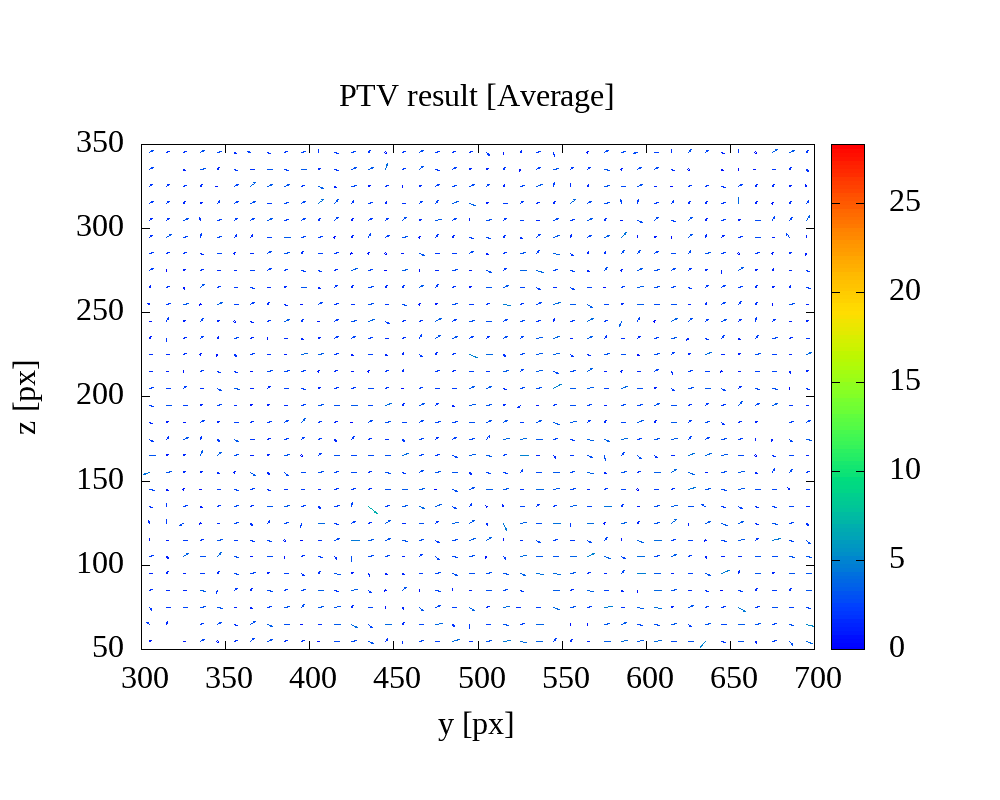
\includegraphics[width=85mm]{../images/uniform_ave.png}
    \caption{時間平均の速度分布 (1000枚分)}
    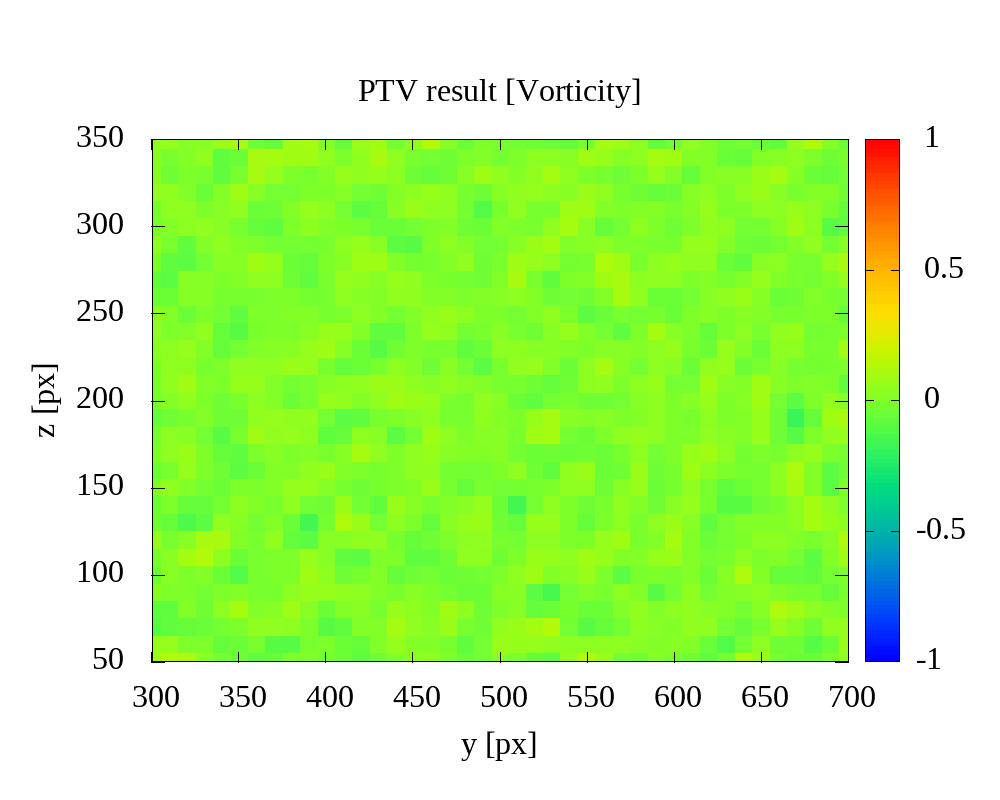
\includegraphics[width=85mm]{../images/uniform_vor.png}
    \caption{渦度分布}
  \end{center}
\end{figure}

Fig.1より,一様流の撮影であるため
速度分布は小さいことがわかる.
また,Fig.2の渦度分布についても
0 周辺の値を持っていることがわかる.\\

\newpage

\subsection{実験結果:タイヤモデル後流}

\begin{figure}[htbp]
  \footnotesize
  \begin{center}
    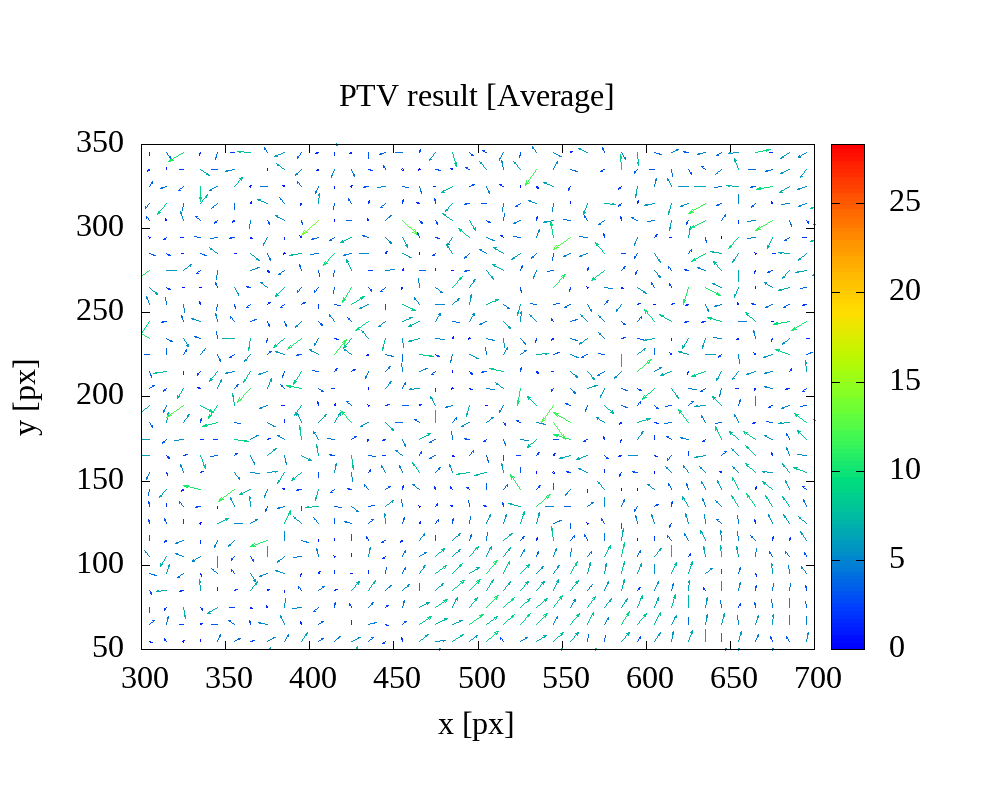
\includegraphics[width=85mm]{../images/rolling_ave.png}
    \caption{時間平均の速度分布 (1000枚分)}
    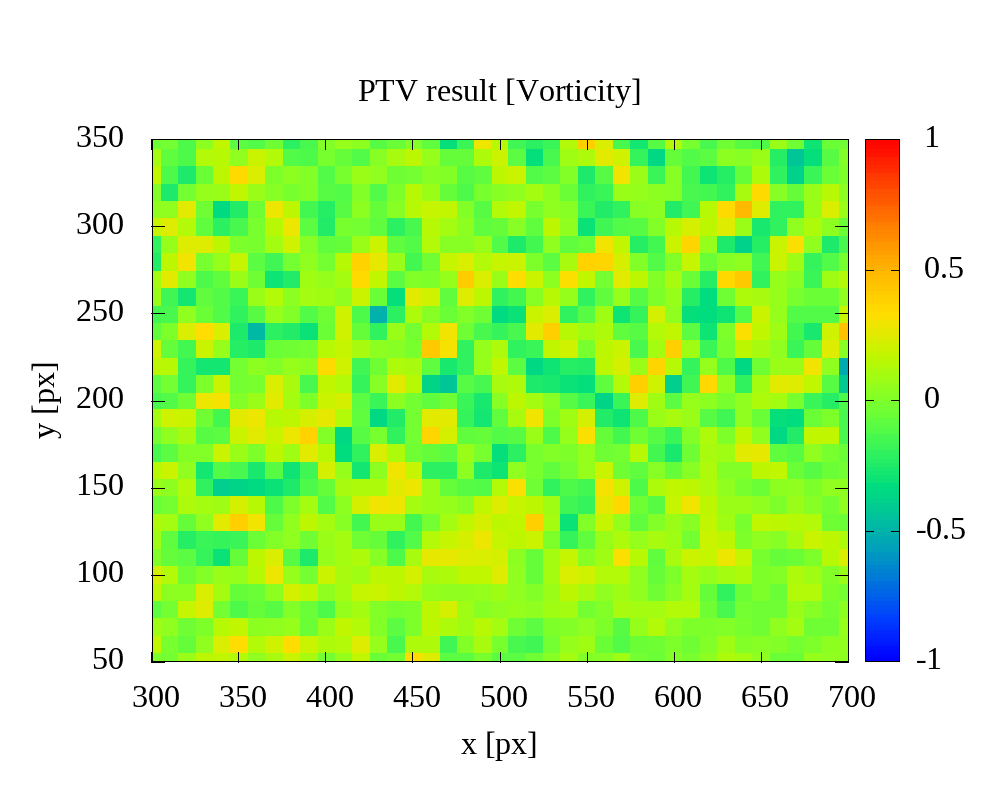
\includegraphics[width=85mm]{../images/rolling_vor.png}
    \caption{渦度分布}
  \end{center}
\end{figure}

Fig.3,Fig.4 はそれぞれ回転タイヤモデルの 50 [mm] 後流における
時間平均の速度分布,渦度分布の算出結果である.
Fig.3より,三角翼後流の結果とは異なり定常的な渦構造は見られない.
また,Fig.4の渦度分布を見ても特徴的な渦度場は確認されない.

\newpage
\section{今後の予定}
\begin{itemize}
  \item 粒子に対応したPTVプログラムの作成
\end{itemize}

\end{document}